\section{Introduction}
%For the past two decades, VHDL and Verilog have governed as hardware description languages (HDLs) for field-programmable gate array (FPGA) and application-specific integrated circuit (ASIC) devices. Originally developed for simulation, these languages have limited synthesizable register-transfer language (RTL) constructs.

%RTLs are very limited due to their explicit expressiveness. For example, vector addition is pipelined, either by coding a registered logic path, or by instancing a pipelined library component. Such components are typically coupled to a specific vendor, device family, or even a given device. Furthermore, clock-latency must be balanced between converging pipelines. Synthesis retiming can assist, provided that the designer places enough registers beforehand.


Low-level hardware description languages (HDLs) such as Verilog and VHDL have been dominating the field-programmable gate array (FPGA) and application-specific integrated circuit (ASIC) domains for decades.
These languages burden designers with explicitly clocked constructs that do not distinguish between design functionality and implementation constraints (e.g., timing, target device).
For example, the register-transfer-level (RTL) constructs of both Verilog and VHDL require designers to explicitly place a register, regardless if it is part of the core functionality (e.g., a state-machine state register), an artifact of the timing constraints (e.g, a pipeline register), or an artifact of the target interface (e.g., a synchronous protocol cycle delay).
%
These semantics narrow design correctness to specific timing restrictions, while vendor library component instances couple the design to a given target device. Evidently, formulating complex portable designs is difficult, if not impossible.
%
Finally, these older languages do not support modern programming features that enhance productivity and correctness such as polymorphism and type safety.

High-level synthesis (HLS) tools such as Vivado HLS~\cite{Vivado2012}, and high-level HDLs such as Bluespec SystemVerilog~\cite{nikhil2004bluespec} and Chisel~\cite{Bachrach2012} attempt to bridge the programmability gap.
While these tools and languages tend to incorporate modern programming features, they still mix functionality with timing and device constraints, or lack hardware construction and timed synchronization control. For example, designs must be explicitly pipelined in Chisel or Bluespec, while a simple task as toggling a led at a given rate is impossible to describe with C++ constructs in Vivado HLS.
Such tools and languages, therefore, fail to deliver a clean separation between functionality and implementation that can yield portable code, while providing general purpose HDL constructs. We explore these gaps further in Section~\ref{sec:related_work}.

In this paper we further extend DFiant~\cite{Port2017}, a modern HDL whose goal is to improve hardware programmability and designer productivity by enabling designers to express truely portable and composable hardware designs.
DFiant decouples functionality from timing constraints (in an effort to end the \emph{"tyranny of the clock"}~\cite{Sutherland2012}). DFiant offers a clean model for hardware construction based on its core characteristics:
\begin{enumerate*}[label=(\roman*)]
\item
  a clock-agnostic dataflow model that enables implicit parallel data and computation scheduling; and
\item
  functional register/state constructs accompanied by an automatic pipelining process, which eliminate all explicit register placements along with their direct clock dependency.
\end{enumerate*} DFiant borrows and combines constructs and semantics from software, hardware and dataflow languages. Consequently, the DFiant programming model accommodates a middle-ground approach between low-level hardware description and high-level sequential programming. 

\begin{figure*}[t]
	\centering
	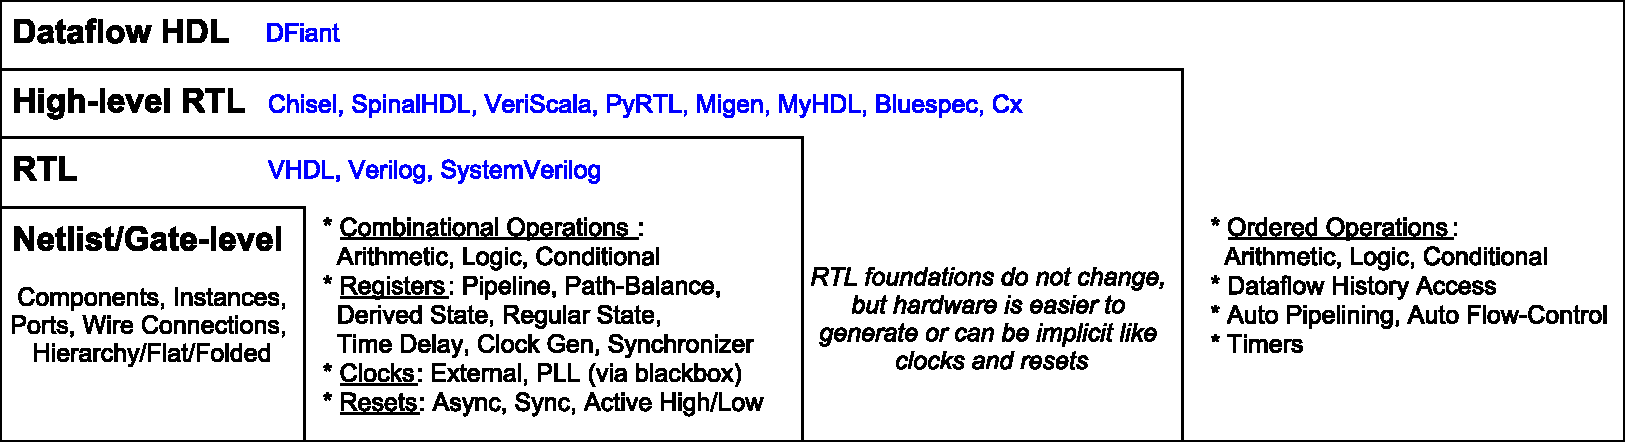
\includegraphics[width=\linewidth]{graphics/motivation.pdf} 
	\captionof{figure}{HDL abstraction layer summary (lowest=netlist, highest=dataflow) \\ DFiant is the first language to support the highest layer, a dataflow HDL.}
	\label{fig:motivation}
\end{figure*}

%\newpage %equivalent to when author names aren't removed
DFiant is implemented as a Scala library and relies on Scala's strong, extensible, and polymorphic type system to provide its own hardware-focused type system (e.g., bit-accurate dataflow types, input/output port types). The library performs two main tasks: the frontend compilation, which translates dataflow variable interactions into a dependency graph; and the backend compilation, which translates the graph into a pipelined RTL code and a TCL constraints file, followed by a hardware synthesis process using commercial tools. Additionally, the graph can be simulated within the Scala integrated development environment (IDE). 

This work focuses on the DFiant language and frontend compiler. DFiant is \emph{not} an RTL language, nor is it a sequential language such as C. The following two sections highlight DFiant's unique semantics by comparing them against modern design language alternatives. For a proof of concept, we implemented a preliminary auto-pipelining backend compiler to compare DFiant and traditional HDL design flows in two test cases: an Advanced Encryption Standard~\cite{pub2001197} (AES) cipher block and an IEEE-754~\cite{IEEE2008} floating point multiplier (FPMul). Future work may delve further into the backend compiler and its HLS potential.


The paper is organized as follows. The next two sections describe DFiant's concurrency and state abstractions, followed by Section~\ref{sec:related_work}, which contrasts DFiant with related work. 
Section~\ref{sec:type_system} details the DFiant type system.
Section~\ref{sec:lzc} provides a real-world DFiant code compilation example.
Section~\ref{sec:evaluation} provides the proof of concept results.
Finally, Section~\ref{sec:conclusion} concludes the paper.




%\newpage
%Interactions between DFiant types lead to hardware construction, while non-DFiant types (e.g. Integer) are considered as constants. 
 

%Modern designs are rich with arithmetic functionality. Surely the designer cannot explicitly pipeline everything manually and must be selective. On one hand, under-pipelining may lead to insufficient performance and redesign iterations. On the other hand, over-pipelining might lead to performance reduction due to limited room for logic and routing, in addition to wasting design time, energy, and device resources. 

%Typical FPGA devices now include clock generators, serializers, PCI express cores, internal memory blocks, external memory interfaces, and many other proprietary modules. Evidently, formulating designs that are transportable across devices and timing variance is difficult, if not impossible. Complex logic design has become a task fit only for experts. 
% The generic code annotations enabling this are cumbersome and limited. 



